\newpage
\section{Der Positive Einfluss des \gls{ESM} auf die Krisenländer}
Die Maßnahmen, die der \gls{ESM} dauerhaft in den Euroländern etablierte, sind nun seit bald 10 Jahren im Einsatz. Um die Entwicklung beurteilen zu können, ist ein Blick in die entsprechenden Statistiken notwendig. Im Fokus liegen dabei nur die Länder, die Kapital aus den verschiedenen Maßnahmen erhalten haben, also Griechenland, Irland, Portugal, Spanien und Zypern, auf Grund des Umfangs dieser Hausarbeit wird außerdem der Blick auf die Verschuldung, das \gls{BIP} pro Kopf und die
Arbeitslosenquote der Länder beschränkt.
\begin{figure}[H]
\begin{center}
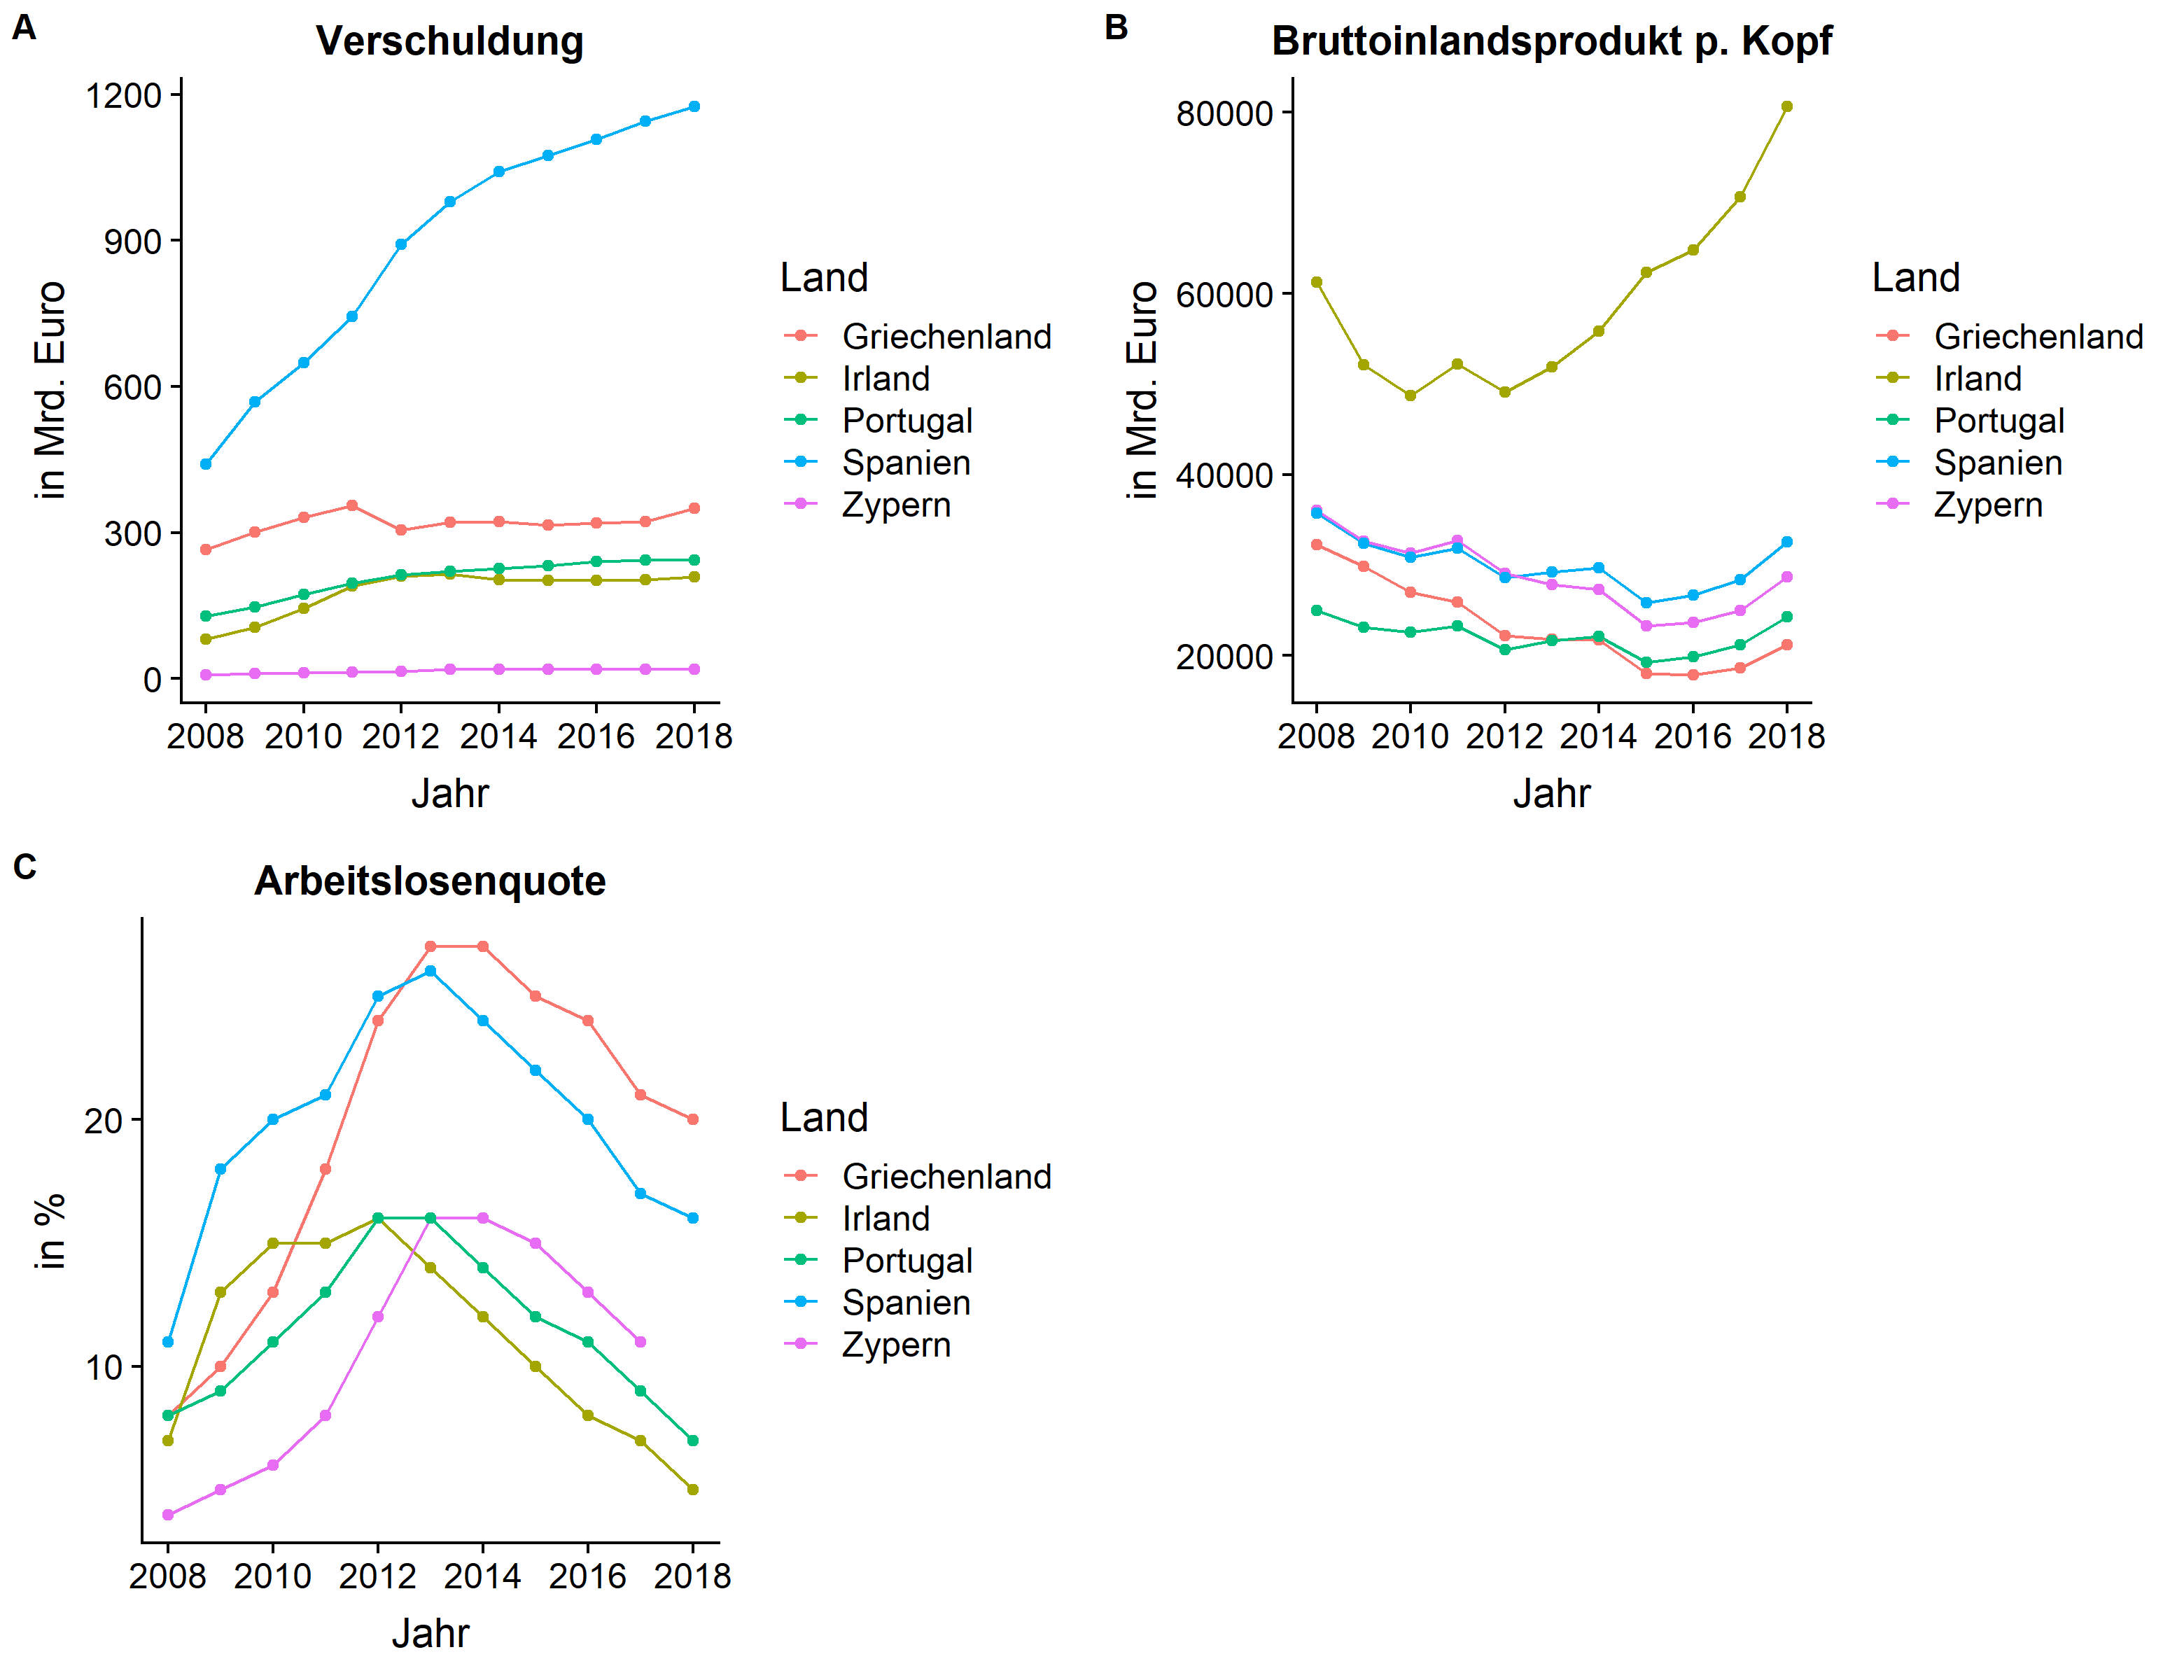
\includegraphics[width=1\textwidth]{grid_plot}
\end{center}%https://www.imf.org/external/pubs/ft/weo/2018/01/weodata/index.aspx
%\caption[Statistik der Länder nach \gls{IMF}\footcite[Aufgerufen am 29.02.2019][man erstelle eine CSV Tabelle mit entsprechenden Quellen]{international_monetary_fund_world_2018}]
\end{figure} %\footnotetext{Aufgerufen am 29.03.2019 über https://www.imf.org/external/pubs/ft/weo/2018/01/weodata/index.aspx -- man erstelle eine CSV-Tabelle mit entsprechenden Optionen}
Abbildung 1 zeigt eine Statistik der ausgewählten Kennziffern in einem 10-Jahres-Zeitraum.
Statistik der Länder nach \gls{IMF}\footcite[Aufgerufen am 29.02.2019][man erstelle eine CSV Tabelle mit entsprechenden Quellen]{international_monetary_fund_world_2018}
\subsection{Staatsverschuldung}
\subsubsection{Griechenland}
\subsubsection{Irland}
\subsubsection{Portugal}
\subsubsection{Spanien}
\subsubsection{Zypern}
\subsection{Bruttoinlandsprodukt}
\subsubsection{Griechenland}
\subsubsection{Irland}
\subsubsection{Portugal}
\subsubsection{Spanien}
\subsubsection{Zypern}
\subsection{Arbeitslosenquote}
\subsubsection{Griechenland}
\subsubsection{Irland}
\subsubsection{Portugal}
\subsubsection{Spanien}
\subsubsection{Zypern}
%Kritiker sehen in den Reformen, die der \gls{ESM} eingeführt hat als Rechtswidrig und Falsch an. Hintergrund ist, dass der Maastricht-Vertrag von 1992 (QUELLE) vorsieht, dass die Länder der \gls{EU} untereinander nicht für die Schulden anderer Mitglieder haftet. Dennoch schaffen es die Reformpakte des \gls{ESM}, die Wirtschaft und den Haushalt wieder in Gang zu setzen.
%Betrachtet man Abbildung 1 fällt auf, dass um das Jahr 2013 jedes Land einen positiven Trend aufweist. Im Falle der Arbeitslosenstatistik zeichnet sich das Bild ganz deutlich: Griechenland schafft es, unter das Niveau im Jahre 2008 zu gelangen
